\documentclass[a4paper]{article}
\usepackage[utf8]{vietnam}
\usepackage{scrextend}
\usepackage{graphicx}


\begin{document}
	
%\chapter{Dữ liệu 1}
Những thông tin vê các giám đốc điều hành các tập đoàn Hoa Kỳ. Bộ dữ liệu gồm 177 quan trắc và 15 biến.

- Chọn mô hình phù hợp nhất giải thích biến phụ thuộc với từng bộ dữ liệu.

- Nêu rõ phương pháp chọn mô hình và lý do chọn phương pháp đó.

- Nói rõ ý nghĩa của mô hình đã chọn.
\subsection*{Tìm hiểu và tiền xử lý dữ liệu}

Một số biến trong bộ dữ liệu kiểu số có đơn vị tính lớn như: $\textit{sales'}$, $\textit{profits}$, $\textit{mktval}$. Nếu đưa những biến này vào phương trình hồi quy có thể dẫn tới hiện tượng bias do tác động của những biến này lên model lấn át những biến khác còn lại như $\textit{age}$, $\textit{ceoten}$.... Nên ta sẽ dùng phương pháp logarit cho 3 biến này trong model tương ứng với 3 biến mới là:  $\textit{lsales"}$ , $\textit{lmktval}$   và $\textit{profmarg}$. (1)


Từ biểu đồ dưới ta thấy ba biến định lượng $\textit{lsales}$, $\textit{lmktval}$ và $\textit{profmarg}$ xảy ra hiện tượng đa cộng tuyến.
Tuy nhiên có xảy ra hiện tượng đa cộng tuyến giữa 2 biến sales và profit luôn (Hình 1)
Tính độ correlation của biến salary với lần lượt 2 biến trên ta có:

\begin{figure}[h!]
	\centering
	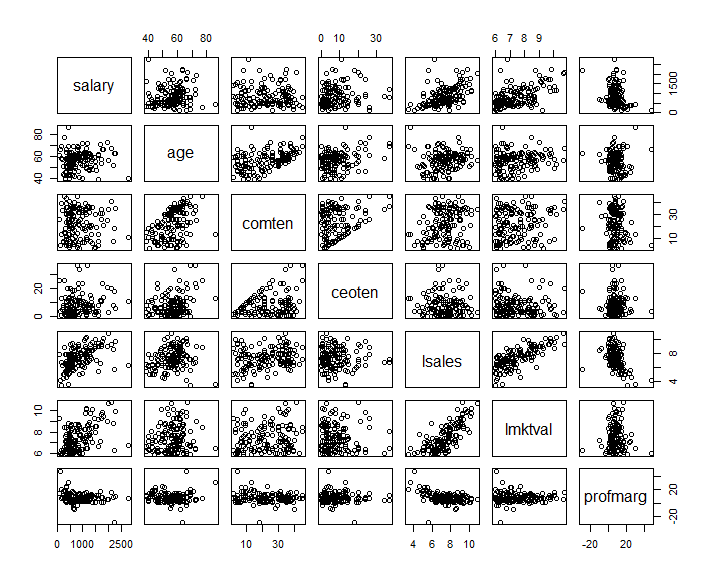
\includegraphics[scale = 0.7]{../Photo Of Result/B1_plotVriables.png}  
	\caption{Mối tương quan giữa các biến}
	\label{ex1:model:1}
\end{figure}

\begin{figure}[h!]
	\centering
	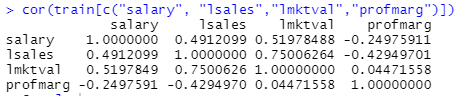
\includegraphics[scale = 0.6]{../Photo Of Result/B1_CorTable.PNG}  
	\caption{Mức độ tương quan giữa biến lsales và promarg Correlation}
	\label{ex1:model:1}
\end{figure}

Xét bảng correlation giữa các biên độc lập với nhau và giữa các biến độc lập với biến phụ thuộc ta thấy: Giữa hai biến $\textit{lmktval}$ và biến $\textit{lsales}$ có mối tương quan rất cao ($\approx$ 0.75). Tuy nhiên biến $\textit{lmktval}$ lại có mối tương quan cao hơn với biến phụ thuộc $\textit{salary}$. Mặt khác giữa biến $\textit{profmarg}$ và $\textit{lsales}$ cũng có mối tương quan cao ($\approx$ -0.42). Nên ta loại bỏ biến $\textit{lsales}$ khỏi danh sách các biến được xét. (2)

Từ (1) và (2) ta có mô hình với đầy đủ các biến cần lựa chọn như sau:

$\textit{salary}$ = $\beta_0$ + $\beta_1$*$\textit{age}$ + $\beta_2$*$\textit{college}$ + $\beta_3$*$\textit{grad}$ + $\beta_4$ * $\textit{comten}$ + $\beta_5$ * $\textit{ceoten}$ + $\beta_6$ * $\textit{lmktval}$ + $\beta_7$ *$\textit{profmarg}$ (1.1)


Thực hiện phân rã hai biến phân loại gồm $\textit{college}$ và $\textit{grad}$ trước khi thực hiện phương pháp chọn biến StepWise tiến với tiêu chuẩn AIC.

Để đánh giá chất lượng mô hình ta chia tâp dữ liệu thành hai phần training và testing với tỷ lệ 80:20 sau đó tiến hành phương pháp chọn biến.

\subsection*{Thực hiện chọn biến bằng phương pháp StepWise tiến và tiêu chuẩn AIC}

\begin{figure}[h!]
	\centering
	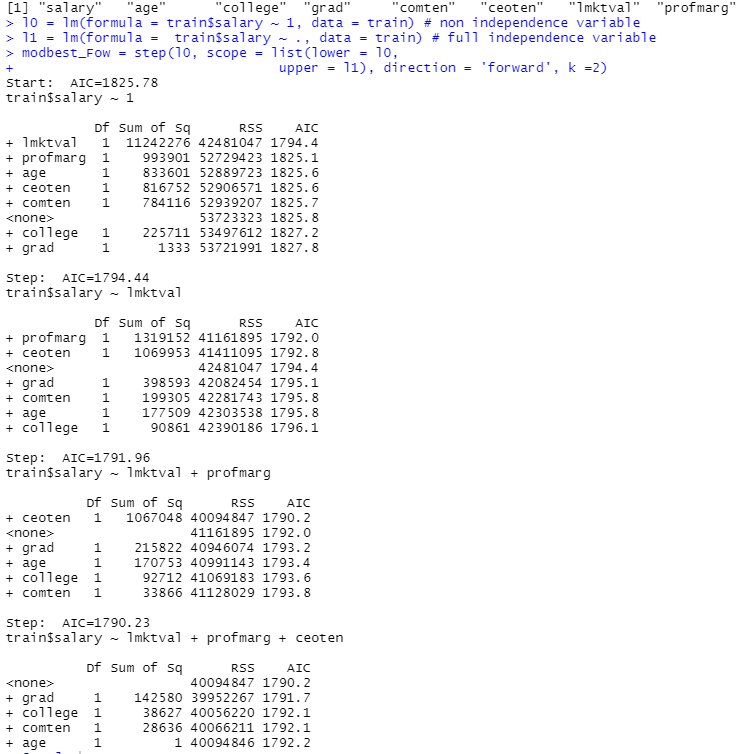
\includegraphics[scale = 0.52]{../Photo Of Result/B1_stepwiseForward.PNG}  
	\caption{Kết quả chọn biến theo phương pháp StepWise tiến với tiêu chuẩn AIC}
	\label{ex1:model:1}
\end{figure}

Tông quan tieu chuẩn AIC thì mô hình tốt là mô hình có giá trị AIC nhỏ nhất. Ở mô hình 1 biến $\textit{lmktval}$ được chọn vào mô hình vì có AIC nhỏ nhất trong tất cả các kết hợp với các biến còn lại. Tương tự AIC được tính cho mô hình thêm biến thứ 2 biến $\textit{ceoten}$ và biến thứ 3 là $\textit{ceoten}$. 

\begin{figure}[h!]
	\centering
	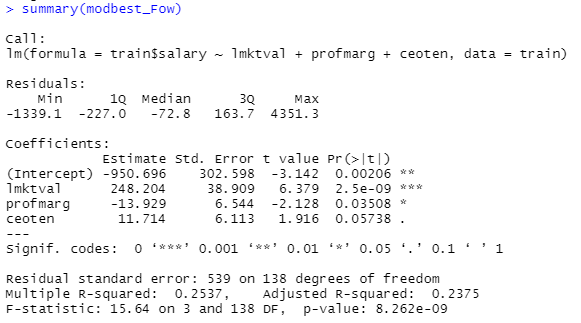
\includegraphics[scale = 0.52]{../Photo Of Result/B1_summary.PNG}  
	\caption{Kết quả hồi quy mô hình với các biên được chọn}
	\label{ex1:model:1}
\end{figure}


Với ba biến trên được chọn mô hình (1.1) trở thành mô hình mới:

$\textit{salary}$ = -950.6 + 248.2 *$\textit{lmktval}$ - -13.9 *$\textit{profmarg}$ + 11.7  *$\textit{ceoten}$  (1.2)

Tuy nhiên ta nhận thấy biến $\textit{ceoten}$ có $\rho_{value} \ge \alpha$ (0.05738 $\ge$ 0.05) nên không có ý nghĩa thống kê trong mô hình.

Ta tiến hành bỏ biến $\textit{ceoten}$ và hồi quy mô hình với hai biến còn lại kết quả thu được từ phần mềm R như bên dưới:

\begin{figure}[h!]
	\centering
	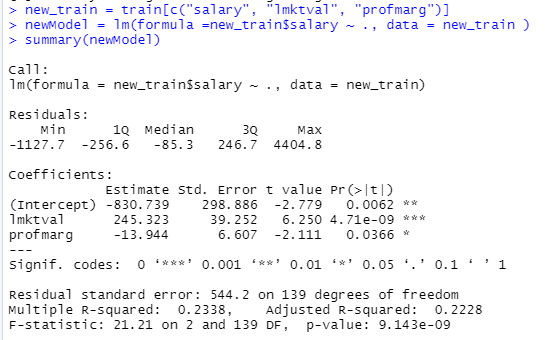
\includegraphics[scale = 0.52]{../Photo Of Result/B1_newsummary.PNG}  
	\caption{Kết quả hồi quy mô hình với hai biến còn lại}
	\label{ex1:model:1}
\end{figure}

Mô hình thống kê mới:

$\textit{salary}$ = -830.7 + 245.3 *$\textit{lmktval}$ -13.9 *$\textit{profmarg}$ + 11.7  (1.3)


Trường hợp này hai biến còn lại có ý nghĩa thống kê. Tuy nhiên mô hình được tạo bởi hai biến này chỉ giải thích được 23 $\%$ kết quả biến phụ thuộc. Nguyên nhân dẫn tới kết quả thấp là do số lượng data ít, các biến giải thích ít không tạo nên mô hình đặc trưng được.



\subsection*{Test trên tập test và nhận xét kết quả}

Thực hiện dự đoán trên tập dữ liệu test từ kết quả mô hình (1.3)  và dùng chỉ số đánh MSE(trung bình sai số bình phương) ta có:

\begin{figure}[h!]
	\centering
	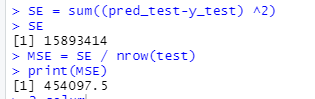
\includegraphics[scale = 0.5]{../Photo Of Result/B1_MSE.PNG}  
	\caption{Chỉ số đo lường kết quả MSE}
	\label{ex1:model:1}
\end{figure}


\end{document}









